\documentclass[12pt,a4paper]{report}

% ---------- Encoding and layout ----------
\usepackage[utf8]{inputenc}
\usepackage[T1]{fontenc}
\usepackage{lmodern}
\usepackage[a4paper,margin=1in]{geometry}
\usepackage{setspace}
\usepackage{parskip}
\usepackage[protrusion=true,expansion=false]{microtype}

% ---------- Maths ----------
\usepackage{amsmath,amssymb,amsthm}

% ---------- Figures / tables ----------
\usepackage{graphicx}
\usepackage{subcaption}
\usepackage{booktabs}
\usepackage{longtable}
\usepackage{array}
\usepackage{float}

% ---------- Code ----------
\usepackage{listings}
\usepackage{xcolor}


\lstset{
    basicstyle=\ttfamily\small,
    breaklines=true,
    frame=single,
    columns=fullflexible
}

% ---------- Hyperlinks ----------
\usepackage[hidelinks]{hyperref}

% ---------- Harvard style ----------
\usepackage[numbers]{natbib}

% ---------- Formatting ----------
\usepackage{titlesec}
\onehalfspacing

% ---------- Title ----------
\title{\textbf{AI-Driven Trade Communication Assistant}\\[0.5em]
\large Final Dissertation}
\author{Xian Diao \\ 20513832}
\date{COMP3003 Individual Dissertation \\ University of Nottingham}

\begin{document}

% =========================
% Title Page
% =========================
\begin{titlepage}
\centering

{\LARGE School of Computer Science\\
University of Nottingham\par}

\vspace{2.5cm}

{\Huge \textbf{AI-Driven Trade Communication Assistant}\par}

\vspace{2.5cm}

{\large Author\\
——\\
20513832\\
scyxd6@nottingham.ac.uk\\
\par}

\vspace{2cm}

{\large Supervised by\\
Paul Tennent\\
paul.tennent@nottingham.ac.uk\par}

\vspace{2cm}

{\large I hereby declare that this dissertation is all my own work, except as indicated in the text.\par}

\vspace{1.5cm}

{\large Date: 14 April 2026\par}

\vfill

\end{titlepage}

% =========================
% Front Matter
% =========================
\cleardoublepage
\pagenumbering{roman}

\chapter*{Abstract}

Small and medium-sized enterprises (SMEs) face significant challenges in international trade, including communication barriers, limited access to standardised documentation, and uncertainty in risk and compliance assessment. This dissertation presents an AI-driven trade communication assistant designed to support SMEs in handling cross-border business interactions.

The system adopts a modular client-server architecture and integrates three core functionalities: communication generation, risk identification, and basic document generation. A large language model is used to generate context-aware responses, supported by structured trade fact extraction and risk analysis. A risk-aware communication mechanism is introduced to ensure that responses reflect both business intent and compliance considerations.

The system was developed through an iterative process involving prompt engineering, system refinement, and pilot testing. A task-based user study was conducted to evaluate system performance across different trade scenarios.

Results indicate that the system generates clear, professional, and contextually appropriate responses, while adapting communication strategies according to identified risk levels. However, limitations remain in handling ambiguous inputs, achieving deeper module integration, and supporting fully standardised documentation.

Overall, this work demonstrates the feasibility of integrating AI-driven communication and risk analysis within a unified framework, and highlights its potential as an assistive tool for international trade.


\section*{Use of Artificial Intelligence Tools}

In this dissertation, AI tools are used solely for supportive purposes.

First of all, AI was used to extensively search for potentially useful literature, then all literatures were independently reviewed by the author, select literatures that can support the arguments.

AI was also userd to conduct a preliminary summary of a large amount of content, to reduce time wastage and improve work efficiency.

In addition, AI was used to help improve formatting and language clarity, particularly in ensuring compliance with academic writing conventions.

All core ideas, system design, implementation, analysis, and conclusions presented in this dissertation are the original work of the author.

%
%\chapter*{Acknowledgements}
%\addcontentsline{toc}{chapter}{Acknowledgements}

\tableofcontents
%\listoffigures
%\listoftables

%\clearpage
%
\pagenumbering{arabic}

% =========================
% Chapter 1
% =========================
\chapter{Introduction}

\section{Project Overview}

This project develops an AI-driven trade communication assistant consisting of three main modules: communication, document generation, and risk analysis.

The communication module is responsible for interacting with large language models (LLMs) to generate responses. The document generation module produces structured business documents such as contracts and invoices. The risk analysis module evaluates incoming messages to identify potential compliance and transaction risks.

\section{Research Context}

Small and medium-sized enterprises (SMEs) play a fundamental role in the global economy, accounting for over 90\% of all firms worldwide and contributing significantly to employment \citep{wto2016, worldbank2020}. Although SMEs show their importance, they remain underrepresented in international trade, reflecting the structural barriers they face when participating in global markets \citep{wto2016,oecd2017}.

In particular, SMEs encounter a range of challenges in cross-border trade, including communication barriers, difficulties in producing standardised business documents, and the complexity of regulatory and compliance requirements \citep{oecd2017, unctad2021}. Although recent advances in artificial intelligence have introduced various tools to support business operations, existing solutions still face significant challenges, including technological complexity, data limitations, and regulatory issues, which hinder their effective integration in practice \citep{ozturk2024}.

Therefore, this project aims to develop a unified system that supports SMEs in multilingual and intercultural communication, automated document generation, and risk identification. By integrating these functionalities, the system aims to enhance efficiency, reduce operational complexity, and facilitate more effective participation in international trade.

\section{Aim and Objectives}

The aim of this project is to develop an intelligent assistant system to support enterprise-level trade. The system is designed to process incoming information from external sources, such as emails and text messages, and assist users in handling business interactions efficiently.

Specifically, the system is expected to:
\begin{itemize}
    \item Automatically interpret incoming messages using natural language processing techniques;
    \item Generate appropriate responses that support business communication using large language models;
    \item Identify and analyse potential risks in the input messages;
    \item Generate standardised business documents based on user requirements and extracted trade information.
\end{itemize}

Through the integration of these functionalities, the system aims to improve communication efficiency, reduce human workload, and enhance risk awareness in international trade scenarios.

\section{Dissertation Structure}

This dissertation is organised into nine chapters, each addressing a specific aspect of the project.

Chapter 2 presents the background and motivation of the project, including the market environment, the challenges faced by SMEs, and the overall project scope. Chapter 3 focuses on real-world problems, analysing key issues encountered in practice and outlining the solutions proposed by this system.

Chapter 4 reviews related work, including existing systems and research on automated communication, document generation, and risk analysis.

Chapter 5 describes the system development in detail, covering design, implementation, and challenges encountered.

Chapter 6 presents pilot testing and system refinement, with a focus on prompt engineering and iterative improvements. Chapter 7 reports the results of the user study, including user feedback and adoption intentions.

Chapter 8 discusses the findings and provides guidelines for future development. Finally, Chapter 9 concludes the dissertation.


% =========================
% Chapter 2
% =========================
\chapter{Background and Motivation}

\section{Challenges in Cross-Border Trade}

SMEs face various barriers in cross-border trade, including information asymmetries, limited market knowledge, and complex business environments, which can hinder effective communication and business relationships \citep{itc2021}.

In addition to communication issues, SMEs often lack the financial resources, digital skills, and technical capabilities required to effectively participate in international trade and digital business environments \citep{unctad2021}.

Furthermore, regulatory complexity presents another significant challenge. SMEs must navigate diverse legal and regulatory frameworks across different countries. The cost and difficulty of understanding and complying with these requirements can act as barriers to market entry and increase operational risk \citep{wto2016,oecd2021}.

\section{SMEs-Specific Constraints}

While these challenges affect enterprises of all sizes, they are particularly significant for SMEs. Compared to large corporations, SMEs typically operate with limited financial resources, smaller workforces, and less access to specialised expertise \citep{oecd2021}.

As a result, SMEs are more vulnerable to operational challenges due to their limited resources and capabilities. In addition, they face higher relative costs when adopting new technologies, as implementing advanced systems often requires technical expertise and financial investment that may not be readily available \citep{oecd2021,mckinsey2023}.

\section{Motivation for an AI-Driven Solution}

Recent advances in artificial intelligence, particularly in natural language processing (NLP) and large language models (LLMs), provide new opportunities to address these challenges. LLMs are capable of understanding unstructured text, generating context-aware responses, and supporting multilingual and intercultural communication.

In addition, AI techniques can facilitate document automation by extracting key information and structuring it into predefined formats. They can also assist in identifying potential risks in communication content, providing early warnings for users.

Despite these capabilities, many existing tools focus on isolated tasks rather than offering an integrated solution. This motivates the development of a unified system that combines communication assistance, document generation, and risk identification.

\section{Project Scope}

This project focuses on the design and development of an AI-driven trade communication assistant tailored for SMEs. The system supports three core functionalities: multilingual communication, risk identification, and document generation.

The communication component interprets incoming messages and generates context-aware responses. The risk analysis component evaluates message content to identify potential compliance and transaction risks. These two components form the primary focus of the system.

In addition, a basic document generation component is implemented to demonstrate the feasibility of producing structured trade documents, such as quotations. This functionality is designed as a supporting feature rather than a fully developed module.

It is important to note that the system does not replace professional legal or regulatory advice. It is developed as an academic prototype and does not include large-scale deployment or real-time regulatory integration.


% =========================
% Chapter 3
% =========================
\chapter{The Real-World Problem}

\section{Problem Definition}

In international trade, SMEs frequently rely on manual processes to handle customer enquiries, interpret message content, and assess transaction risks. A typical workflow involves receiving incoming messages, analysing the content, identifying the underlying intent and potential risks, and determining an appropriate course of action, such as responding to the enquiry or requesting further information. In addition, SMEs also need to provide the relevant documents if required.

This process is time-consuming and prone to error. Communication is often conducted in non-native languages, which increases the likelihood of misunderstandings and reduces response quality.

Another key issue is the fragmentation of tools. Existing solutions typically address only a single aspect of the workflow, such as translation or document generation. As a result, users must switch between multiple systems, reducing efficiency and increasing cognitive load.

Therefore, the core problem addressed in this project is how to support SMEs in handling cross-border trade communication through an integrated system that combines message understanding, response generation, risk identification, and document creation.

\section{Representative Use Cases}

To illustrate the real-world relevance of the problem, this section presents several representative use cases in which SMEs may benefit from intelligent support for trade communication, risk awareness, and related documentation tasks.

\subsection*{Use Case 1: Out-of-Hours Customer Enquiries}

In cross-border trade, customer inquiries may come from different time zones and sometimes fall outside the working hours of recipient. In certain cases, these messages may be urgent, and a delayed response could reduce customer satisfaction or lead to a missed business opportunity.

For SMEs with limited staff availability, it may not always be possible to monitor and respond to such messages. In this situation, an intelligent assistant could help by generating a brief and appropriate preliminary reply, acknowledging the enquiry and maintaining communication until a fuller response can be provided.

\subsection*{Use Case 2: Large Volumes of Incoming Messages}

SMEs may receive a large number of incoming emails or enquiries, not all of which have the same business value or level of risk. Some messages may represent legitimate opportunities, while others may be vague, low-value, or potentially risky.

Manually reviewing and prioritising these messages can be time-consuming, particularly for small teams. In such situations, a support system that helps identify lower-risk and potentially higher-value messages could assist users in deciding which enquiries to review first. A draft replies will also be prepared in advance, the user may then approve or revise them, reducing the overall workload associated with repetitive communication tasks.

\subsection*{Use Case 3: Unfamiliar Trade Documentation Requirements}

When SMEs enter unfamiliar business areas, such as new import or export activities, they may lack experience with the standard forms of documentation expected in international trade. Preparing quotations, invoices, or similar business documents may therefore become a source of uncertainty and inefficiency.

In such cases, access to structured and standardised document templates could provide useful guidance and reduce the likelihood of formatting or content errors. A system that offers template-based support or basic document generation may therefore help users handle documentation tasks more confidently. More advanced functions, such as document review and compliance checking, remain potential directions for future development.

\section{Key Requirements}

\subsection{Functional Requirements}

The system should be able to:
\begin{itemize}
    \item Interpret incoming messages and extract key information, including user intent and contextual details;
    \item Identify and analyse potential risks associated with the message content;
    \item Generate professional and context-aware responses based on the identified intent and risk level;
    \item Support different response strategies, such as proactive engagement, cautious clarification, or restricted replies in high-risk scenarios;
    \item Provide basic support for generating standardised trade documents;
    \item Support multilingual input and output.
\end{itemize}

\subsection{Non-Functional Requirements}

\begin{itemize}
    \item \textbf{Usability:} The system should be easy to use for non-expert users;
    \item \textbf{Efficiency:} Message processing and response generation should be performed within a reasonable time;
    \item \textbf{Reliability:} The system should produce consistent and coherent outputs;
    \item \textbf{Scalability:} The design should allow future extension of functionalities;
    \item \textbf{Explainability:} Risk identification results should be interpretable and understandable to users.
\end{itemize}

\section{Challenges in Practice}

To meet these requirements, developing such a system in real-world scenarios would encounter several practical challenges.

\subsection{Ambiguity in User Input}

User messages are often incomplete, vague, or inconsistently structured. In many cases, key information such as product specifications, quantities, or delivery requirements may be missing or only implicitly expressed. This makes it difficult for the system to accurately interpret user intent and extract reliable information, increasing the risk of inappropriate or irrelevant responses.

\subsection{Multilingual and Cross-Cultural Complexity}

Cross-border communication frequently involves multiple languages and cultural contexts. Messages may include mixed languages, informal expressions, or non-standard grammar, which complicates interpretation. Furthermore, generating appropriate responses requires not only accurate language processing but also sensitivity to cultural norms, tone, and business etiquette.

\subsection{Regulatory and Compliance Uncertainty}

International trade is subject to diverse and evolving regulations, including export controls, sanctions, and product-specific restrictions. Identifying potential risks from textual input alone is inherently uncertain, as regulatory requirements vary across regions and may not be explicitly stated in the message. The system must therefore balance sensitivity and specificity when flagging risks, avoiding both underreportings and false positives.

\subsection{Limitations of Large Language Models}

Although large language models provide powerful capabilities for language understanding and generation, they are not inherently reliable. Issues such as hallucination, inconsistency, and lack of domain-specific knowledge may lead to inaccurate or misleading outputs. In a business context, such errors can have significant consequences, making it essential to carefully control how LLM-generated responses are used.

\subsection{Integration of Multiple Functionalities}

The system is required to combine message understanding, risk analysis, and response generation within a unified workflow. Ensuring smooth interaction between these components presents a significant challenge, particularly in maintaining consistency between extracted information, risk assessment results, and generated responses. Poor integration could lead to unexpected outputs and reduce reliability of system.


% =========================
% Chapter 4
% =========================
\chapter{Related Work}

\section{Digitalisation and AI in International Trade}

Digital technologies, including artificial intelligence (AI), are reshaping international trade by enabling new forms of digital interaction and facilitating cross-border data flows \citep{unctad2021}. AI has the potential to enhance trade processes through improved decision-making and automation, thereby supporting more efficient and data-driven business operations \citep{wto2025,oecd_ai_trade}.

\section{AI Applications in Trade Operations}

AI has been applied in several areas of trade operations. In document processing, automation reduces administrative burden and improves efficiency \citep{oecd_doc}. Similarly, in communication, natural language processing enables multilingual interaction and supports more effective business communication.

AI is also used in logistics optimisation and risk assessment, where predictive models can identify patterns and support decision-making. These applications demonstrate the versatility of AI in trade-related tasks \citep{ozturk2024}.

\section{AI Adoption Challenges in SMEs}

Despite these advantages, AI adoption remains limited in SMEs due to resource constraints, lack of expertise, and related capability gaps \citep{oecd2021}. Additional organisational and technical challenges may further impede effective integration into business processes.

\section{Research Gap}

Existing solutions typically focus on individual tasks, such as communication, document generation, or risk analysis, rather than providing integrated support.

There is a lack of systems that combine these functionalities into a unified workflow. This project addresses this gap by proposing an integrated AI-driven system that supports multiple aspects of trade communication.


% =========================
% Chapter 5
% =========================
\chapter{Developing Process}

\section{Overall Development Strategy}

The development of the AI-Driven Trade Communication Assistant followed an iterative and modular strategy. Given the complexity of integrating natural language processing, risk analysis, and document generation into a single system, a phased development approach was adopted.

The initial phase focused on building a minimal viable system capable of processing user input and generating basic responses using a large language model (LLM). This was followed by the introduction of structured trade fact extraction, enabling the system to standardise user inputs and support more reliable downstream processing.

In subsequent iterations, additional modules were developed and integrated, including risk identification, document generation, and user data management. Each module was implemented and tested independently before being incorporated into the overall system pipeline. Continuous refinement was carried out based on observed system behaviour, particularly in prompt engineering and response quality.

The final system reflects a layered architecture in which communication, compliance, and document generation functionalities are tightly integrated, enabling end-to-end support for international trade scenarios.

\section{System Design}

\subsection{System Architecture}

The system adopts a client-server architecture consisting of a lightweight web frontend and a Python-based backend built using FastAPI. The backend is organised into multiple functional modules, including communication, document generation, risk identification, user management, and data storage.

The current frontend operates primarily as a development-oriented interface rather than a fully developed user workspace. In practice, the system is mainly used to input trade-related requests through simple controls or console-style interaction and inspect the resulting outputs, including generated responses and risk annotations. Communication between the frontend and backend is handled through RESTful APIs.

The backend integrates a large language model via API calls, which is responsible for natural language understanding, response generation, and content structuring. The architecture is designed to be modular, allowing individual components to be extended or replaced without affecting the overall system.

Figure~\ref{fig:architecture} illustrates the overall system architecture, highlighting the interaction between the frontend interface, backend services, and supporting data layers. It shows how user inputs are routed through API endpoints to core processing modules, and how outputs and logs are managed within the system.

\begin{figure}[H]
    \centering
    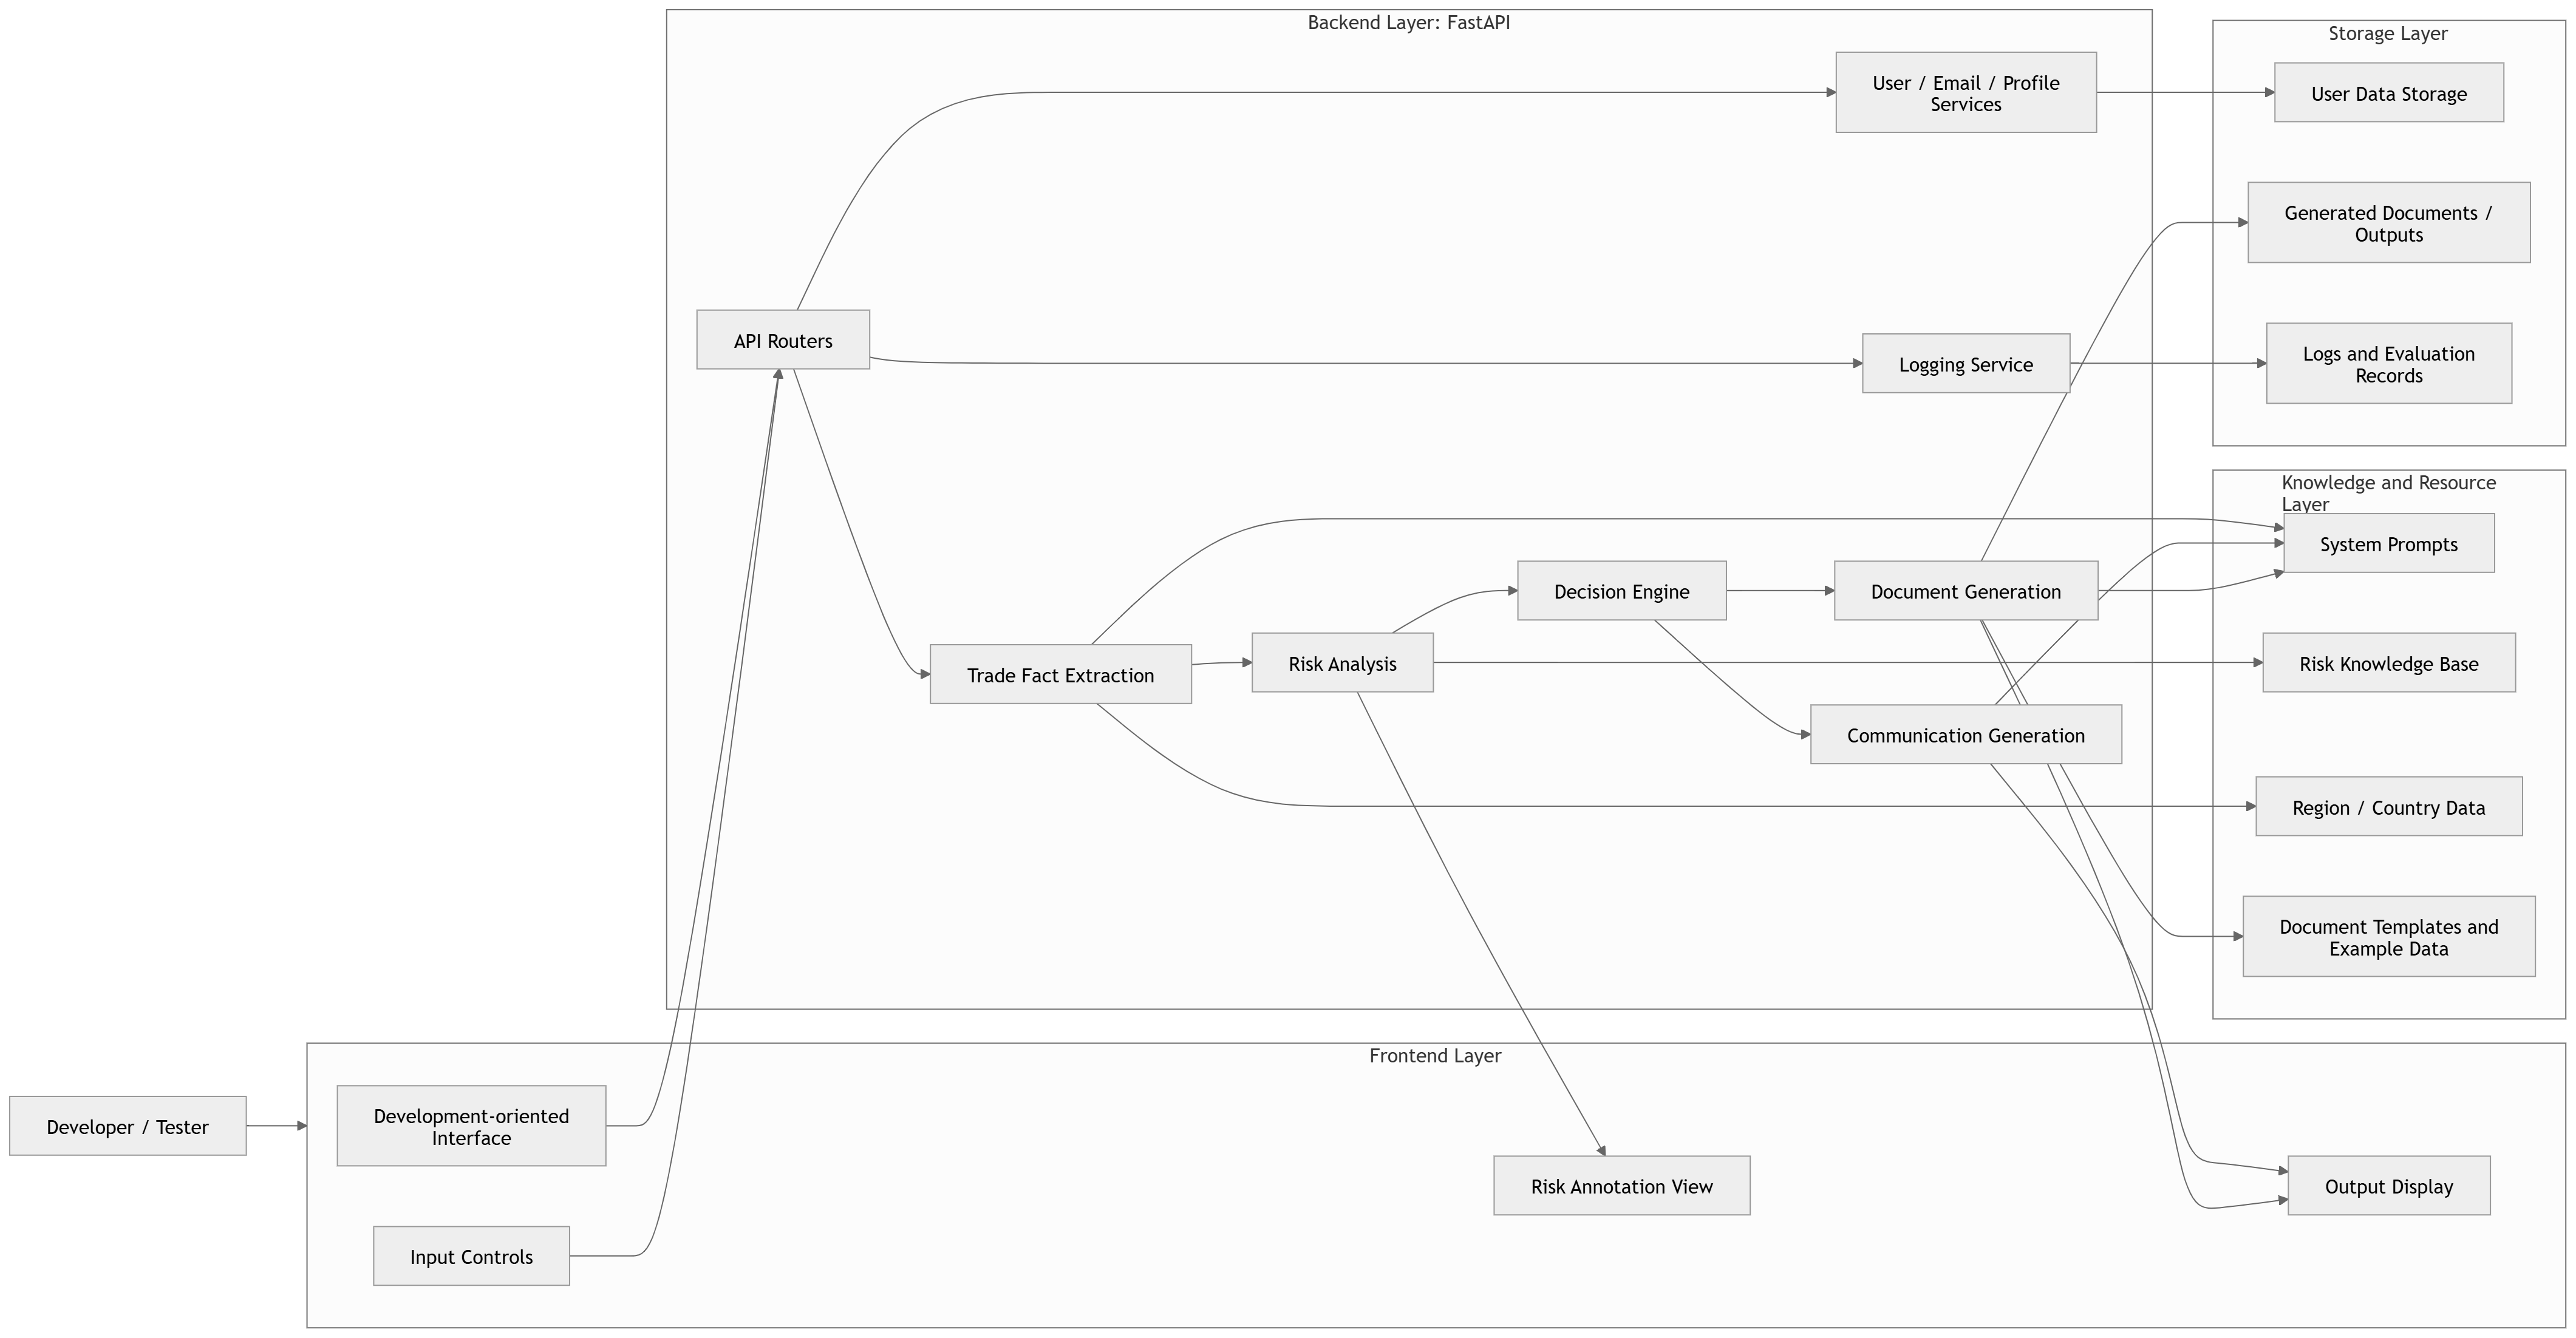
\includegraphics[width=\linewidth]{projectstructure.png}
    \caption{Overall System Architecture}
    \label{fig:architecture}
\end{figure}

\subsection{Data Flow}

The system processes user input through a structured pipeline, ensuring that both semantic understanding and compliance considerations are incorporated into the final output. As shown in Figure~\ref{fig:dataflow}, the workflow follows a sequential yet modular process:

\begin{enumerate}
    \item \textbf{User Input}: The user provides a message or document request via the frontend interface.
    
    \item \textbf{Trade Fact Extraction}: The input is analysed to extract structured information such as product details, language, and region.
    
    \item \textbf{Risk Identification}: The system evaluates the extracted information and original input to assign risk tags and severity levels.
    
    \item \textbf{Decision Routing}: Based on the identified risks, the system determines whether to proceed normally, provide warnings, or restrict certain outputs.
    
    \item \textbf{Response Generation}: The LLM generates a reply based on the information extracted from input and the risks identified by the previous module.
    
    \item \textbf{Output Rendering}: The result is returned to the frontend, where it is displayed along with risk annotations.
\end{enumerate}

This pipeline ensures that communication generation is informed by both structured data and compliance considerations, enabling the system to balance usability with risk awareness.

\begin{figure}[H]
    \centering
    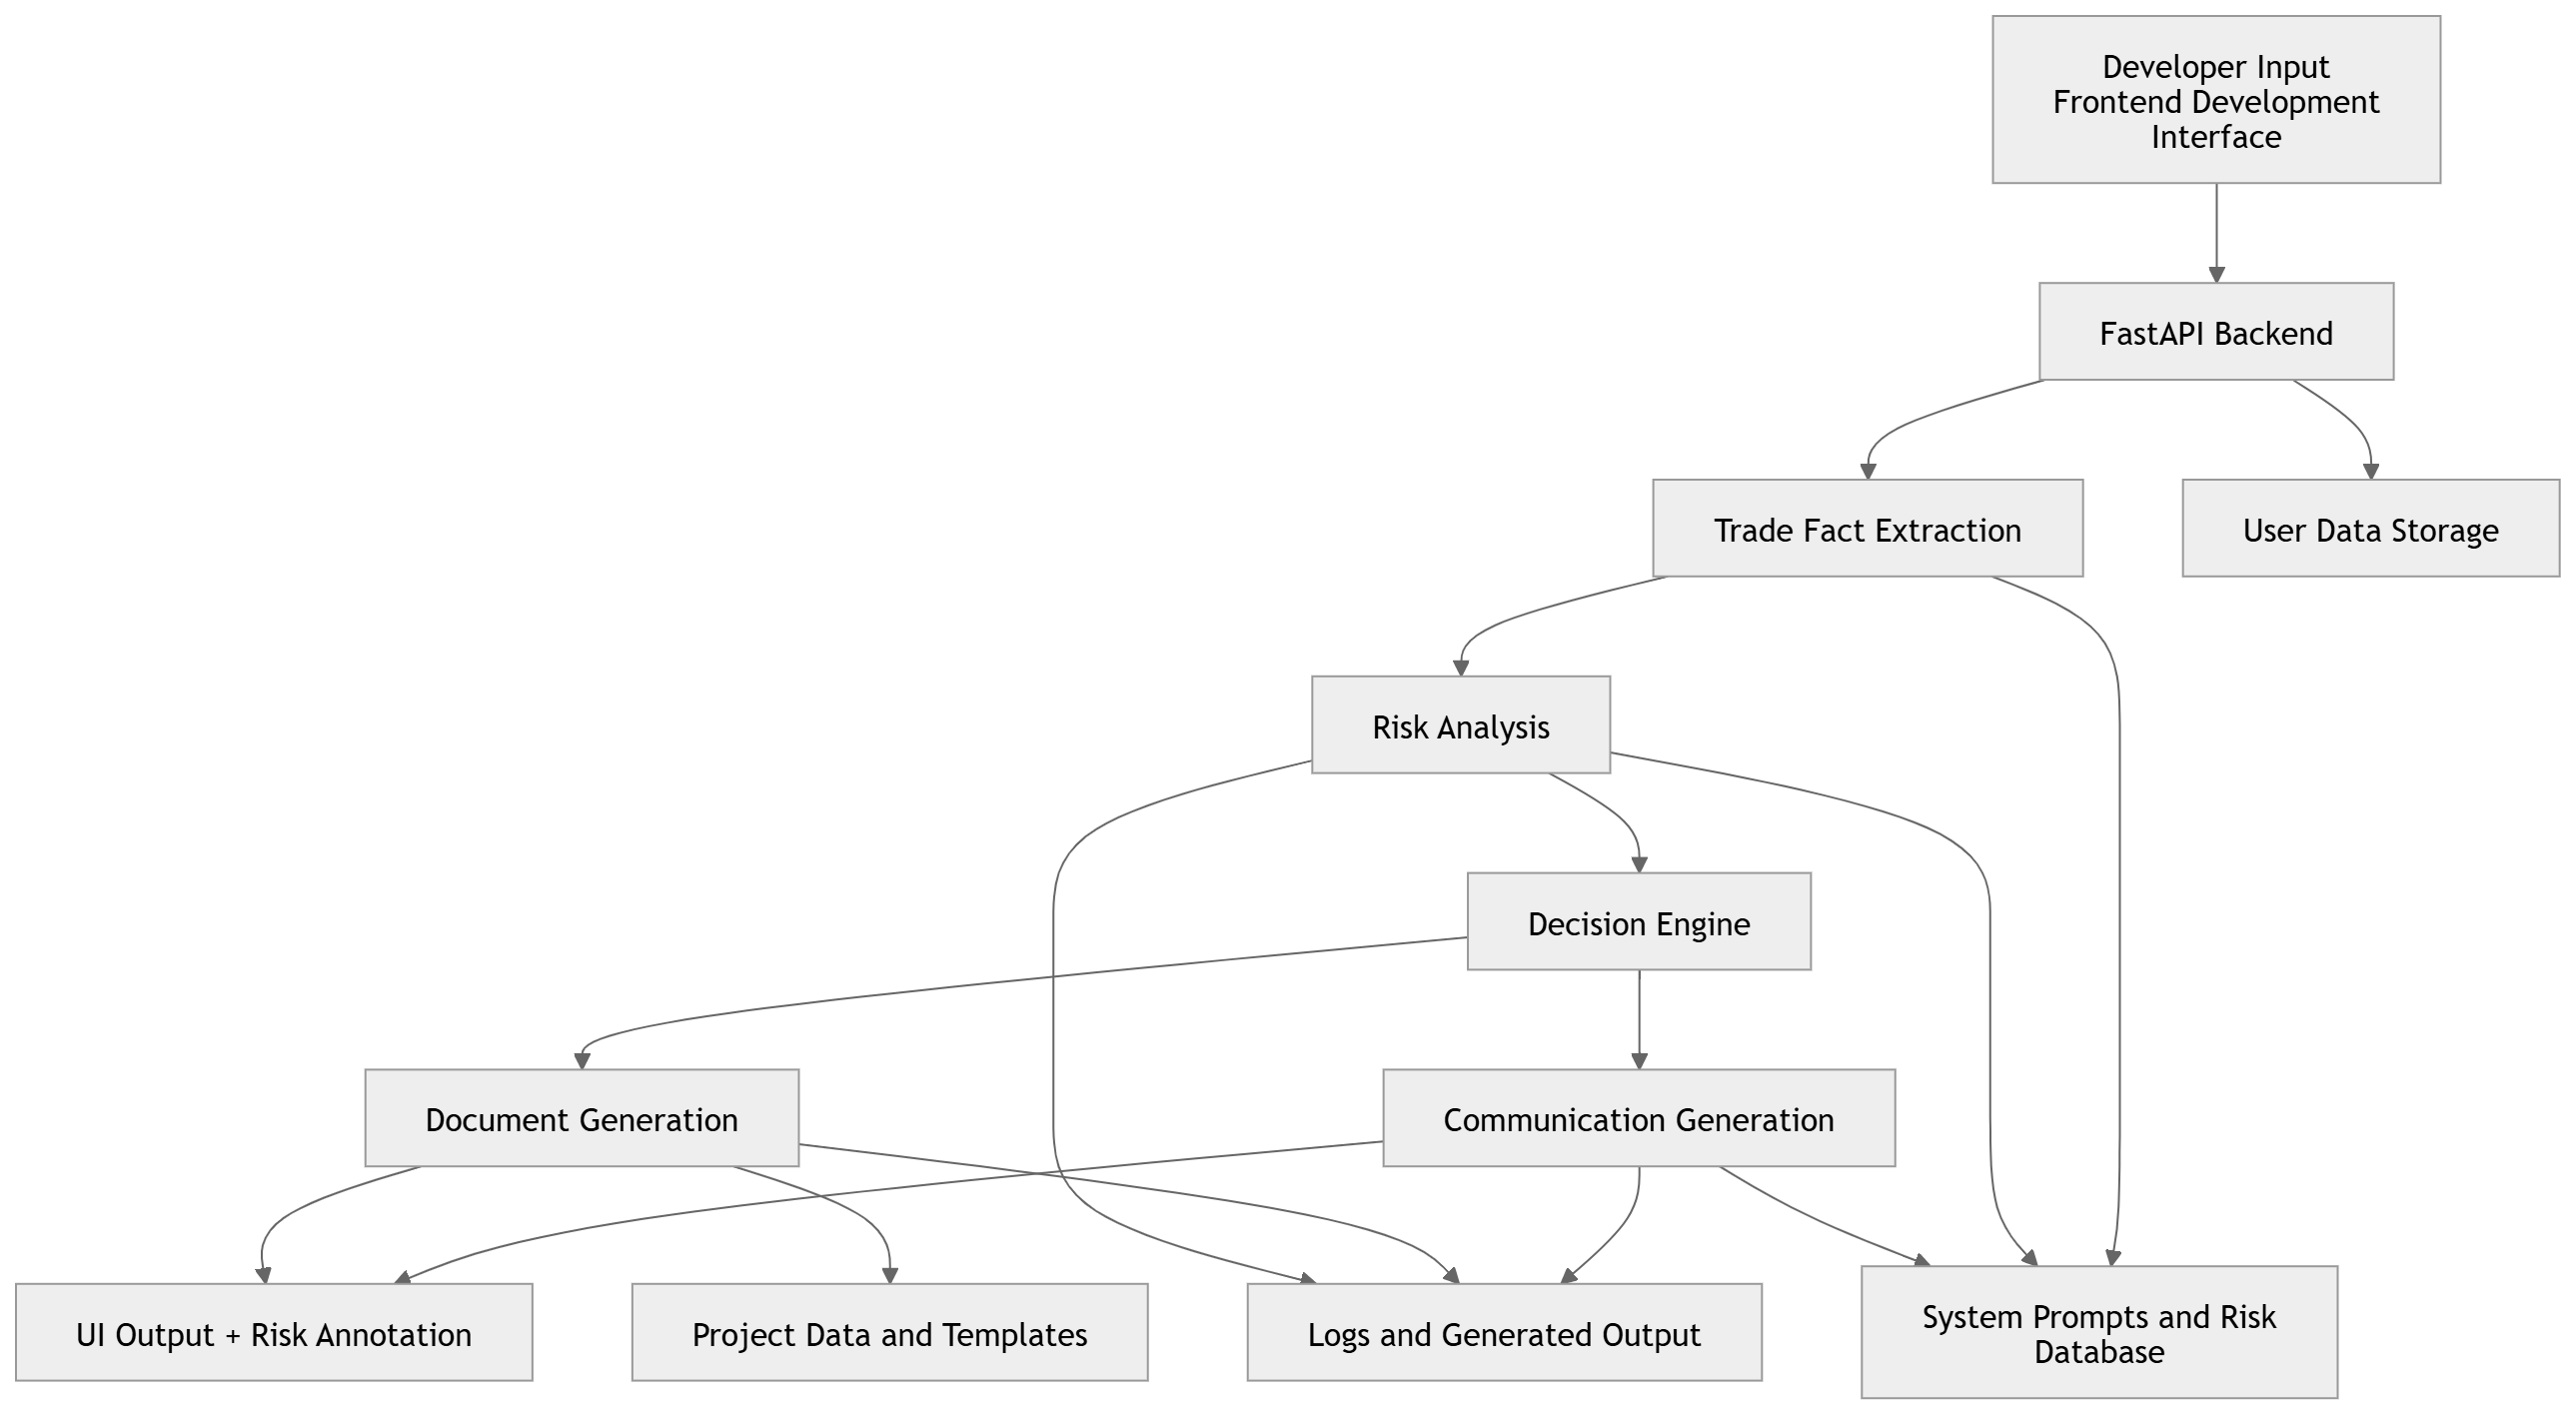
\includegraphics[width=\linewidth]{dataflow.png}
    \caption{System Data Flow}
    \label{fig:dataflow}
\end{figure}

\subsection{Module Design}

The system is composed of several core functional modules, supported by additional system-level components.

\textbf{Core Functional Modules}

The primary functionality of the system is implemented through three main modules:

\textbf{Communication Module:} Responsible for generating replies to user messages. It incorporates contextual information such as language, region, and communication style to produce responses that are coherent and appropriate for business interactions.

\textbf{Risk Identification Module:} Analyses inputs to detect potential compliance and transaction risks. It assigns multiple risk tags with associated severity levels and computes an overall risk level using a weighted aggregation approach.

\textbf{Document Generation Module:} Provides basic support for generating structured trade documents, such as quotations and contracts. It supports parameter-based generation and template-assisted creation, producing outputs in PDF format. At the current stage, this module serves primarily as a proof of concept rather than a fully standardised documentation system.

\textbf{Supporting System Modules}

In addition to the core functional modules, the system includes several supporting components that enable system operation and data management:

\textbf{Data Storage Module:} Manages user data, generated emails, and documents using a lightweight JSON-based storage mechanism, enabling persistent tracking of interactions.

\textbf{User Interface Module:} Provides a development-oriented interface for submitting requests, inspecting generated outputs, and viewing risk annotations during testing and evaluation.

\section{Implementation}

\subsection{Technology Stack}

The system is implemented using the following technologies:

\begin{itemize}
    \item \textbf{Backend:} Python with FastAPI, providing RESTful API endpoints and asynchronous request handling.
    \item \textbf{Frontend:} HTML, CSS, and JavaScript, implementing a lightweight and responsive user interface.
    \item \textbf{LLM Integration:} OpenAI API, used for natural language understanding and generation.
    \item \textbf{Data Storage:} JSON-based file storage, enabling a simple and portable persistence layer.
    \item \textbf{Document Generation:} PDF generation using backend processing and template support.
\end{itemize}

This technology stack was chosen to balance development efficiency, flexibility, and system scalability.

\subsection{Communication Module}

The communication module forms one of the core components of the system and is responsible for generating context-aware business responses. It is implemented as an API endpoint that accepts user messages together with contextual parameters such as language, region, and communication intent.

Prompt templates are used to guide the large language model in producing structured and professional replies. In addition, the system incorporates automatic detection of communication style, enabling it to distinguish between informal enquiries and formal business correspondence.

A key feature of this module is its integration with structured trade facts and risk signals. Extracted information and identified risk tags are embedded into the prompt context, ensuring that generated responses reflect both business requirements and compliance considerations. This allows the system to move beyond generic text generation towards risk-aware and context-sensitive communication.

\subsection{Risk Identification Module}

The risk identification module represents another core component of the system, providing structured analysis of potential compliance and transaction risks.

The module evaluates both the original user input and the extracted trade facts to assign multiple risk tags. Each tag is associated with a severity level (high, medium, low), capturing different dimensions of risk such as regulatory constraints, transaction patterns, and communication signals.

Rather than relying on a single maximum value, the system computes an overall risk level using a weighted aggregation of all detected tags. This approach enables a more nuanced assessment, where multiple moderate risks can collectively influence the final judgement.

The resulting risk information is returned as structured data and visualised in the frontend using colour-coded labels, improving interpretability and supporting informed decision-making.

\subsection{Document Generation Module}

The document generation module provides supplementary functionality for producing structured trade documents. It supports multiple document types, including quotations and basic contracts, and allows users to input structured information such as product details, pricing, and payment terms.

For certain document types, template files or reference materials can be used to guide content generation. The backend processes the input and produces a PDF output, which is returned as a downloadable file together with a descriptive summary.

At the current stage, this module serves primarily as a proof of concept, demonstrating the feasibility of automated document generation. It does not yet provide fully standardised or legally validated documentation, and further development is required to support comprehensive template libraries and compliance checking.

\subsection{Frontend and Interaction Design}

The frontend is implemented as a lightweight, development-oriented interface that facilitates interaction with the backend system. Rather than a fully featured end-user application, it primarily serves as a testing and inspection environment for system functionality.

Users interact with the system through a console-style input panel, where trade-related requests can be entered and submitted. The interface supports two main interaction modes—communication and document generation—which can be switched via a tab-based layout. As shown in Figure~\ref{fig:mainUI}, the main interface consists of an input area for user messages and a corresponding output panel where generated responses are displayed.

\begin{figure}[H]
    \centering
    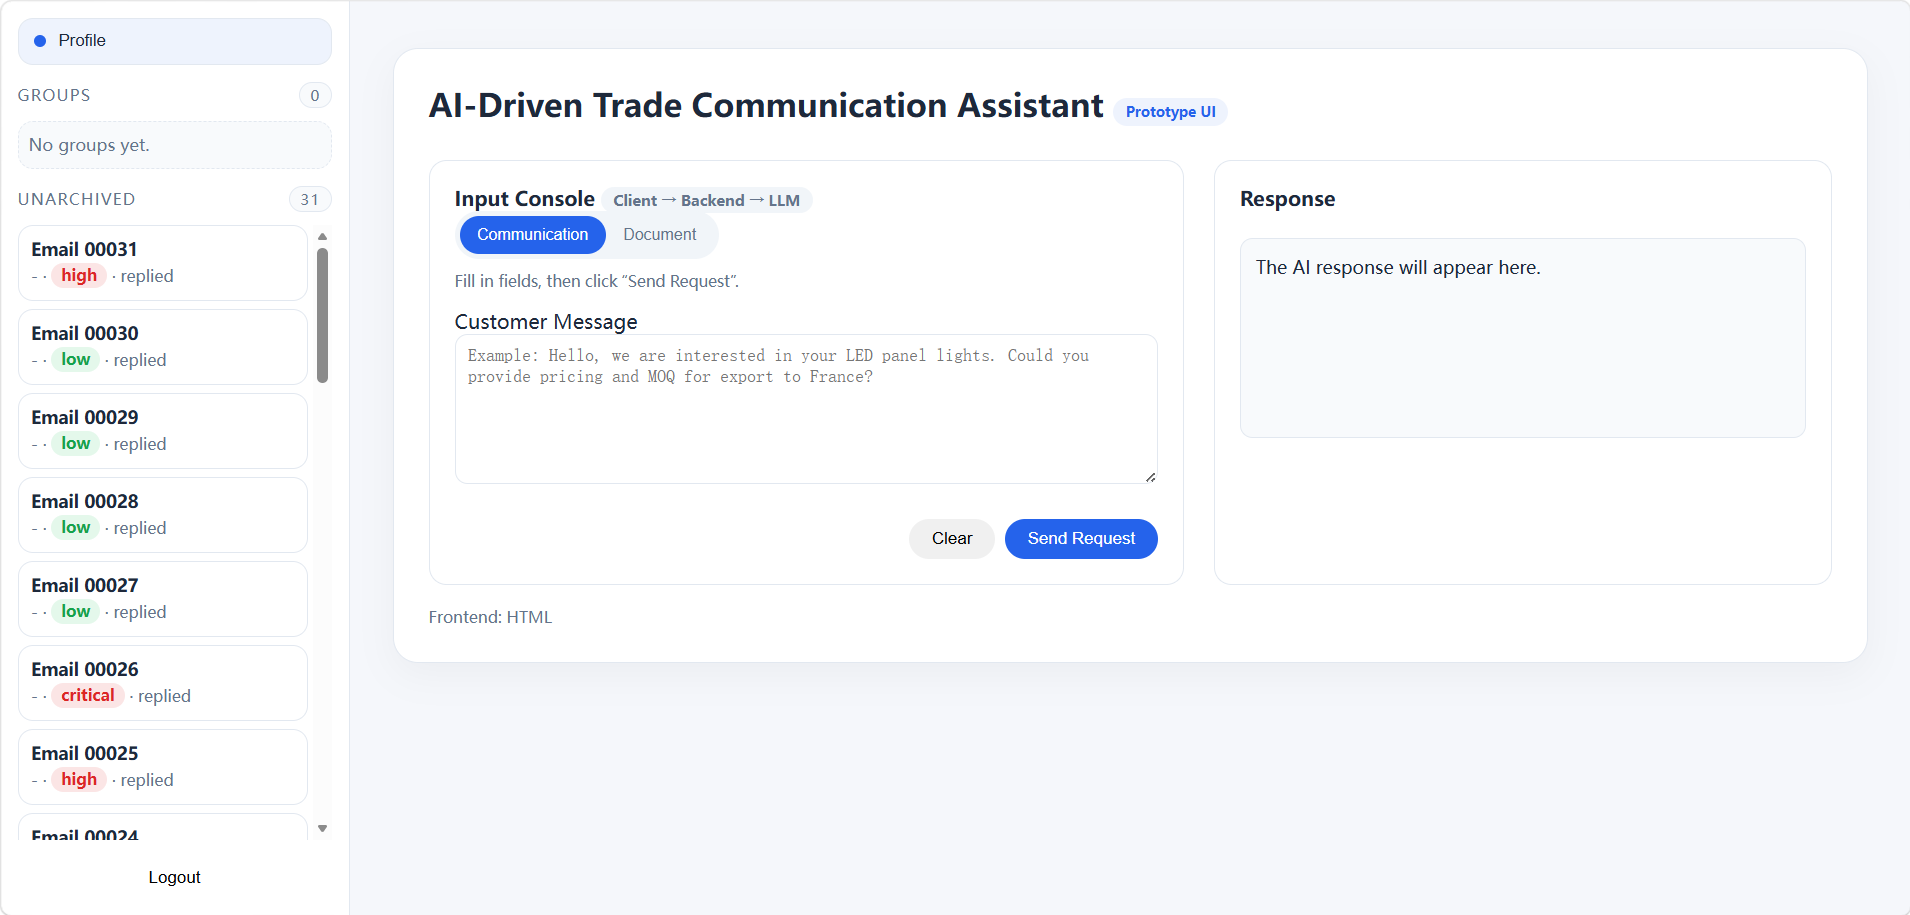
\includegraphics[width=\linewidth]{mainUI.png}
    \caption{Main frontend interface with input console and response panel}
    \label{fig:mainUI}
\end{figure}

In addition to the input–output interaction, the system provides a sidebar for browsing previously generated emails and accessing user profile information. Individual email entries can be selected to view detailed interaction records, including the original message, generated reply, and associated risk annotations.

Figure~\ref{fig:emailUI} illustrates the email detail view. Risk information is presented using colour-coded tags alongside an overall risk level, enabling users to quickly interpret potential compliance or business concerns. This design supports transparency and helps users understand how risk signals influence system behaviour.

\begin{figure}[H]
    \centering
    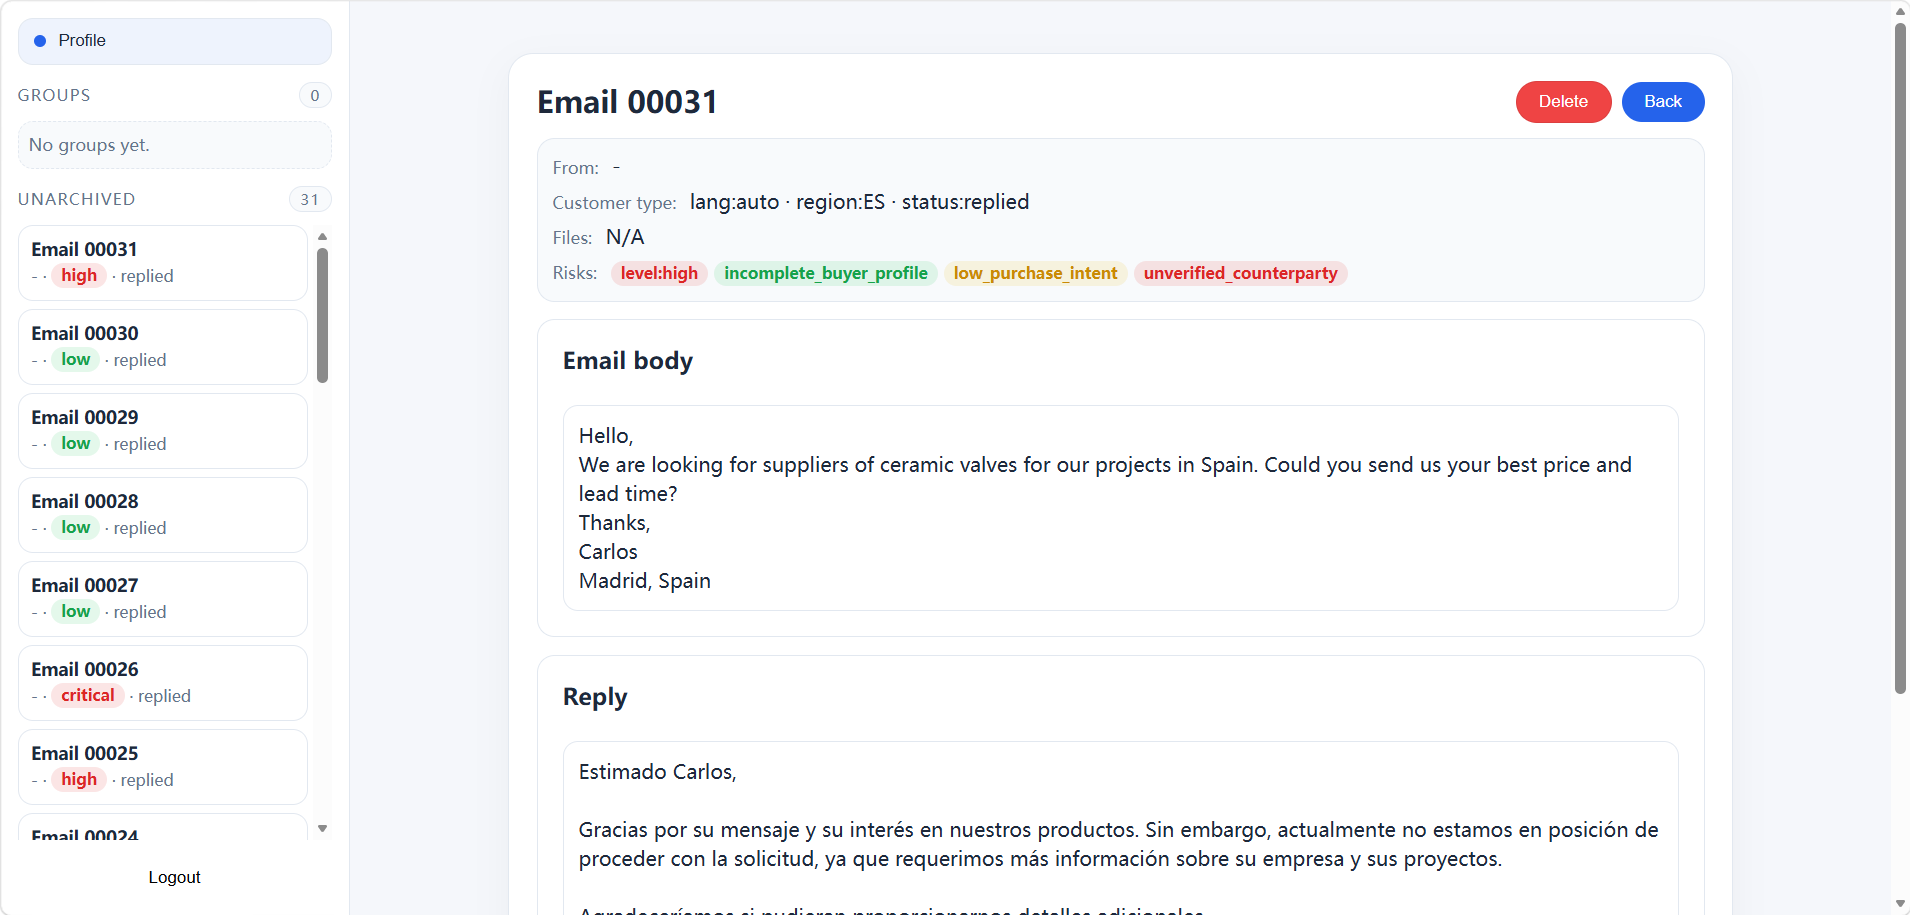
\includegraphics[width=\linewidth]{emailUI.png}
    \caption{Email detail view with generated reply and risk annotations}
    \label{fig:emailUI}
\end{figure}

Authentication is implemented using a token-based mechanism, and all frontend–backend communication is conducted through centralised RESTful API calls, ensuring a clear and consistent interaction flow.

\section{Development Challenges}

Several challenges were encountered during the development process.

One major challenge was handling ambiguous and unstructured user input. This was addressed by introducing a trade fact extraction layer to standardise inputs before further processing.

Another challenge involved balancing response quality and compliance. Without proper constraints, the LLM could generate responses that overlooked potential risks. This issue was mitigated by integrating risk analysis into the generation pipeline.

Ensuring consistent document formatting was also difficult, particularly when supporting different document types and templates. Iterative refinement of generation logic and template handling was required to achieve stable outputs.

Last but not least, managing system complexity and module interaction required careful architectural design. A modular approach was adopted to ensure that each component could be developed and tested independently while maintaining overall system coherence.

% =========================
% Chapter 6
% =========================
\chapter{Pilot Testing and System Refinement}

\section{Purpose of Pilot Testing}

Pilot testing was conducted to evaluate the behaviour of the system in realistic trade communication scenarios and to identify limitations in prompt design, response generation, risk identification and decision-making logic. 

The main purpose of the tests was not to measure final performance, but to refine the system by observing how it responded to different inputs, including incomplete enquiries, cross-border communication, and varying risk conditions. Particular attention was given to whether the system could generate responses that were not only correct, but also practical, natural, and directly usable in real business contexts.

\section{Initial System Behaviour}

In its early version, the system demonstrated basic functionality in extracting information, assessing risk, and generating replies. It was capable of identifying certain high-risk scenarios and producing responses in multiple languages.

However, despite these capabilities, the overall behaviour of the system was not sufficiently stable or aligned with requirements. Responses often appear unnatural, overly general, or unhelpful in advancing collaboration. In addition, the interaction between risk assessment and reply generation was not well controlled, leading to unpredictable outcomes.

\section{Observed Problems}

Through pilot testing, several recurring issues were identified:

\begin{itemize}
    \item \textbf{Inconsistent tone}: The system sometimes produced overly direct or unnatural responses, especially in high-risk scenarios, where replies could appear abrupt or unfriendly.
    
    \item \textbf{Missing business details}: Many test inputs contained limited information, which caused the system to frequently trigger risk flags such as "incomplete\_buyer\_profile", leading to overly cautious responses.
    
    \item \textbf{Overly generic replies}: Early outputs often resembled template-based responses and lacked specificity, reducing their usefulness in real communication.
    
    \item \textbf{Unstable formatting}: Responses occasionally included placeholder expressions such as \texttt{[Your Name]} or improperly structured greetings, which exposed the artificial nature of the output.
    
    \item \textbf{Risk judgement issues}: Although risk labels are correctly generated in many cases, their impact on response behaviour is inconsistent. High-risk situations can sometimes lead to overly rigid refusals, while medium-risk situations lack a clear direction for responses.
\end{itemize}


\section{Prompt Refinement Process}

To address the issues identified during pilot testing, a systematic prompt refinement process was carried out. This process combined iterative testing, manual inspection of generated outputs, and targeted adjustments to both prompt design and system-level logic.

Rather than relying on a single round of optimisation, refinement was conducted as a continuous loop: test cases were executed, outputs were analysed for errors or undesirable patterns, and prompts were revised accordingly. In cases where prompt-level control was insufficient, additional mechanisms such as post-processing were introduced to ensure output reliability.

\subsection{Refinement Criteria}

The refinement process was guided by a set of criteria reflecting both technical correctness and practical usability:

\begin{itemize}
    \item \textbf{Accuracy}: Responses should correctly reflect the content of the enquiry and any extracted trade information.
    
    \item \textbf{Clarity}: Outputs should be easy to understand and free from ambiguous or placeholder expressions.
    
    \item \textbf{Professional tone}: All responses should maintain a polite and formal tone appropriate for business communication.
    
    \item \textbf{Structural consistency}: Replies should follow a coherent email structure, including greeting, body, and closing.
    
    \item \textbf{Compliance awareness}: Risk signals should influence decision-making without compromising professionalism.
    
    \item \textbf{Naturalness}: Responses should resemble human-written emails rather than AI-generated templates.
\end{itemize}

In addition, particular attention was given to the interaction between these criteria. For example, improving compliance awareness should not lead to overly rigid or unnatural responses, and enforcing structure should not reduce linguistic naturalness. This required balancing multiple objectives during prompt design.

\subsection{Before-and-After Examples}

Early versions of the system frequently produced outputs containing placeholder text or unnatural phrasing. For example:

\begin{quote}
Dear [Your Name], \\
Thank you for your enquiry. Please provide more details.
\end{quote}

Such outputs were unsuitable for direct use, as they exposed template artefacts and required manual editing.

After refinement, the system generated more natural and context-aware responses:

\begin{quote}
Dear Sir or Madam, \\

Thank you for your enquiry regarding our products. We would be pleased to explore potential cooperation. Could you kindly provide further details regarding your required quantity and intended application?
\end{quote}

In this improved version, placeholder expressions are eliminated, the greeting follows standard business conventions, and the response provides a clearer and more cooperative communication strategy. 

This example illustrates how prompt refinement, combined with additional control mechanisms, improves both the linguistic quality and practical usability of the generated outputs.

\section{Refined System Version}

The refined system incorporates a series of prompt-level and architectural improvements developed through the pilot testing process.

Prompt templates were externalised into configuration files, improving modularity and enabling rapid iteration without requiring modifications to the core codebase. In addition, response generation was enhanced to eliminate placeholder expressions. Beyond prompt-level constraints, a post-processing mechanism was implemented within the LLM client to detect and remove or replace any remaining placeholder patterns, ensuring that outputs are immediately usable.

The system adopts a default formal email style, removing unnecessary user controls such as tone selection. This simplifies the interface while ensuring consistent response behaviour. Localisation capability was further improved by enabling the system to infer the customer’s region and generate replies in the corresponding language, thereby supporting context-aware cross-cultural communication.

Greeting generation was standardised through simple rules: when a personal name is available, it is used; otherwise, a generic form such as “Dear Sir or Madam” is applied. This prevents the incorrect use of company names as personal identifiers.

A structured risk-aware response strategy was introduced, in which tone remains consistently polite while decision behaviour varies according to risk level:
\begin{itemize}
    \item Low-risk cases proactively promote cooperation;
    \item Medium-risk cases request additional information;
    \item High-risk cases issue polite refusal while preserving the possibility of future engagement.
\end{itemize}

Finally, the test dataset was refined to include more complete and realistic business information, thereby reducing noise caused by missing data and improving the reliability of evaluation.

Overall, these refinements improved the system’s stability, consistency, and practical usability, enabling it to generate professional and context-aware business communication suitable for real-world applications.

% =========================
% Chapter 7
% =========================
\chapter{User Study}

\section{Study Design}

To evaluate the effectiveness of the proposed AI-driven trade communication assistant, a task-based user study was conducted. The study aimed to assess both user expectations and perceptions of system-generated responses in realistic trade communication scenarios.

Two questionnaires were designed, each containing three distinct email scenarios. The questionnaires featured different email contents, covering a range of scenarios with varying risk levels from low to critical.

For each scenario, participants were required to complete two stages:

\begin{itemize}
    \item \textbf{Stage 1 (Expectation Elicitation):} Participants reviewed an incoming email and assessed its risk level, as well as their expected response strategy.
    
    \item \textbf{Stage 2 (System Evaluation):} Participants were then shown the AI-generated reply for the same email and asked to evaluate its quality and appropriateness.
\end{itemize}

This design enables a direct comparison between human judgement and system behaviour, providing insight into the alignment between user expectations and AI-generated responses.

A total of 14 participants completed the study. Participation was voluntary, and participants were informed about the purpose of the study. No personal or sensitive data was collected. Although the sample size was relatively small, it is appropriate for an exploratory evaluation aimed at identifying qualitative trends rather than statistical significance.

\section{Data Collection Procedure}

The questionnaires were distributed online and completed independently by participants. Each participant evaluated three scenarios within one questionnaire.

All participants followed the same evaluation process. First, they analysed the incoming email and formed their own judgement regarding risk and response strategy. They then evaluated the AI-generated reply using structured criteria.

Both quantitative and qualitative data were collected. Likert-scale questions captured structured evaluations across predefined criteria, while open-ended responses provided additional insights into user perceptions.

The full questionnaire and example scenarios are provided in Appendix A. The collected responses are included in the supplementary materials.

\section{Evaluation Criteria}

The evaluation focused on key aspects of effective international trade communication:

\begin{itemize}
    \item \textbf{Relevance}: Whether the response addressed the enquiry appropriately.
    
    \item \textbf{Clarity}: Whether the response was clear and well-structured.
    
    \item \textbf{Tone Appropriateness}: Whether the response was polite, professional, and culturally suitable.
    
    \item \textbf{Completeness}: Whether sufficient information was provided.
    
    \item \textbf{Practicality}: Whether the response was useful and actionable.
    
    \item \textbf{Risk Handling}: Whether the response appropriately reflected the risk level.
\end{itemize}

Participants also provided overall feedback on system usefulness and their willingness to adopt the system.

\section{Results}

\subsection{Scenario-Based Performance}

The results show that the system demonstrates adaptive behaviour across different risk levels.

In low-risk scenarios (well-defined business enquiries with clear company identity), the system consistently generated professional, complete, and cooperative responses. These responses aligned closely with participant expectations and were generally rated highly across all evaluation criteria.

In medium-risk scenarios (incomplete buyer information or initial enquiries), the system effectively balanced helpfulness and caution. It provided relevant information while requesting additional details, reflecting a strategy similar to that proposed by participants in the expectation stage.

In high-risk scenarios (hazardous product enquiries or incomplete verification), the system correctly identified potential risks and adopted a more cautious approach. Responses typically avoided direct commitment and requested further clarification, which aligns with safe business practices.

In critical-risk scenarios (suspicious payment methods, urgency pressure, or scam-like patterns), the system successfully detected multiple risk signals and flagged them appropriately. However, the generated responses tended to remain neutral and verification-focused rather than explicitly rejecting the request. This indicates a gap between accurate risk detection and sufficiently strong response strategies.

\subsection{Cross-Scenario Comparison}

Across all six scenarios, a clear pattern emerges: the system is capable of adjusting its communication strategy according to the inferred risk level.

This adaptive behaviour is particularly evident in the transition from low-risk to medium-risk scenarios, where the system shifts from cooperative responses to information-seeking strategies. In higher-risk cases, it further transitions to cautious and non-committal replies.

However, the distinction between high-risk and critical-risk responses is less pronounced. While risk classification is accurate, the response strategies do not always fully reflect the severity of the situation. This suggests that the mapping between risk level and response behaviour can be further refined.

\subsection{User Feedback Analysis}

Quantitative results indicate generally positive evaluations across multiple criteria. All ratings were collected using a 5-point Likert scale, where 1 indicates strong disagreement and 5 indicates strong agreement.

\begin{figure}[H]
	\centering
	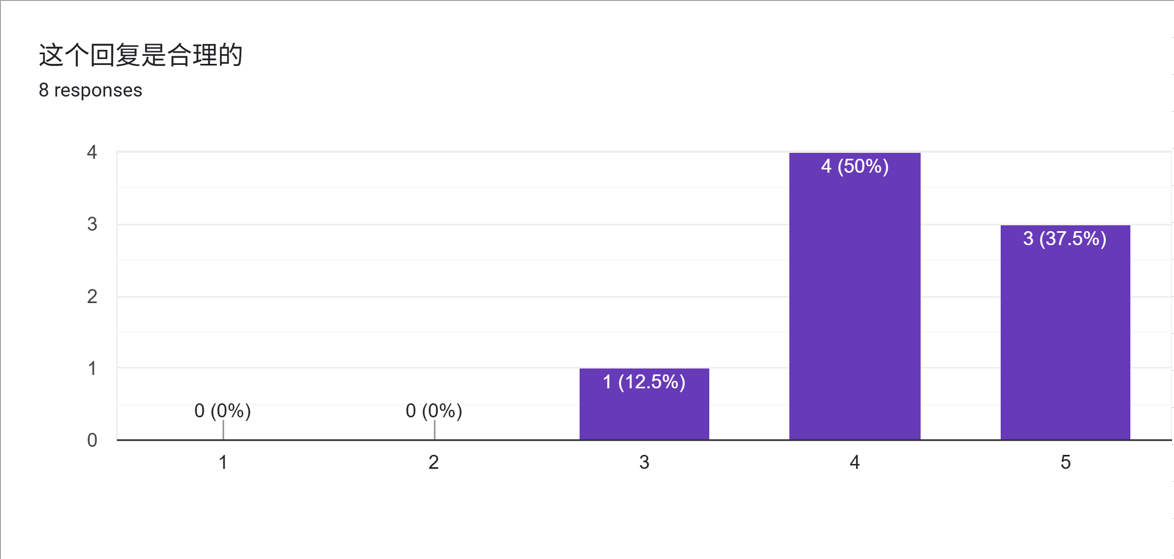
\includegraphics[width=0.45\linewidth]{reasonable.png}
	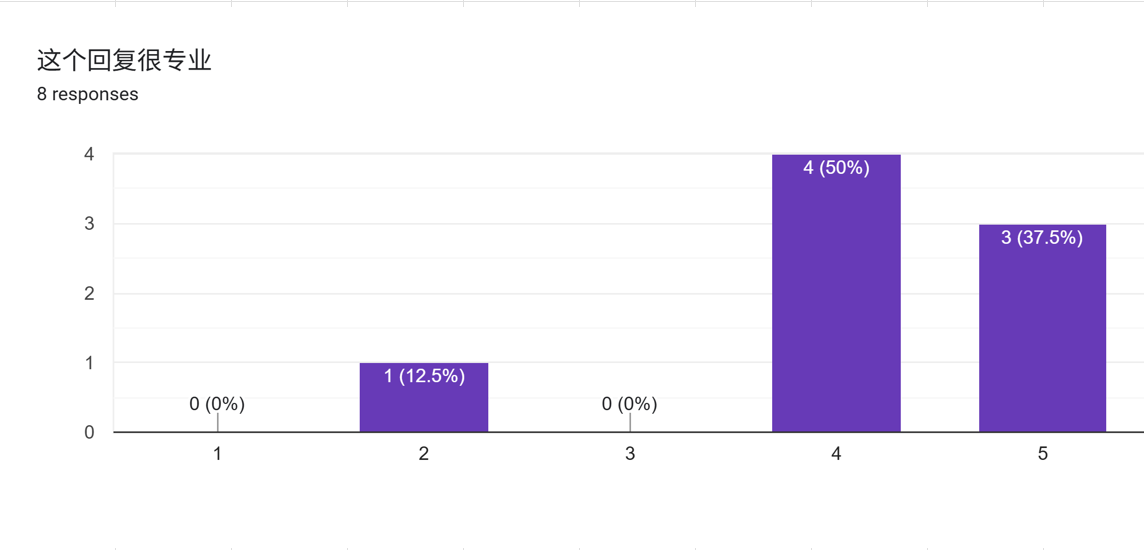
\includegraphics[width=0.45\linewidth]{professional.png}
	
	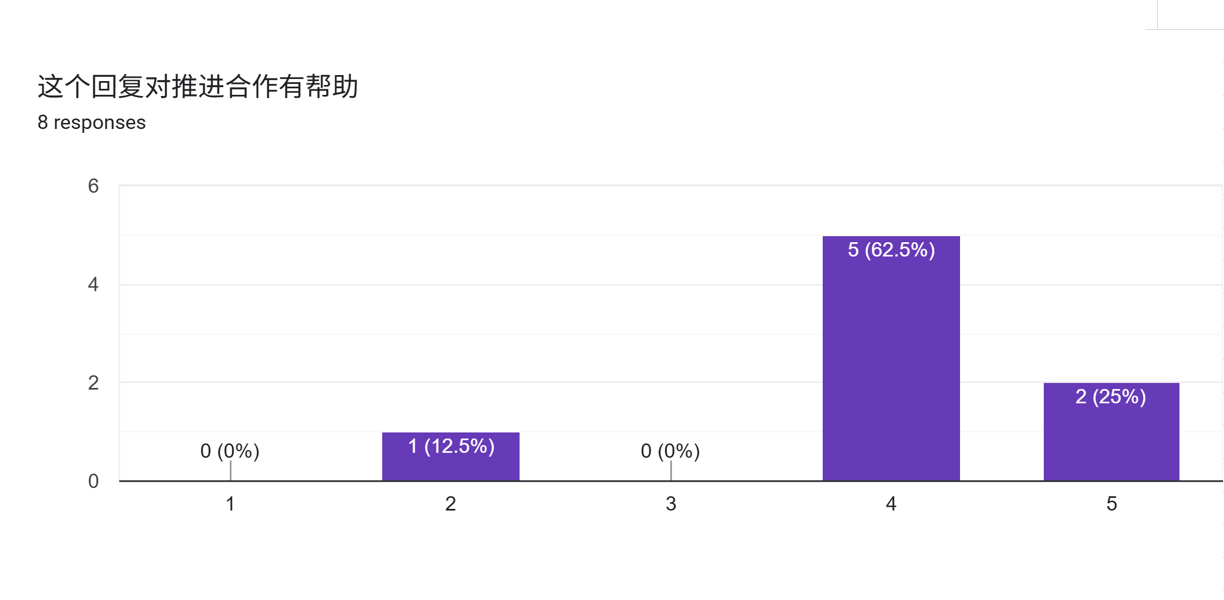
\includegraphics[width=0.45\linewidth]{helpful.png}
	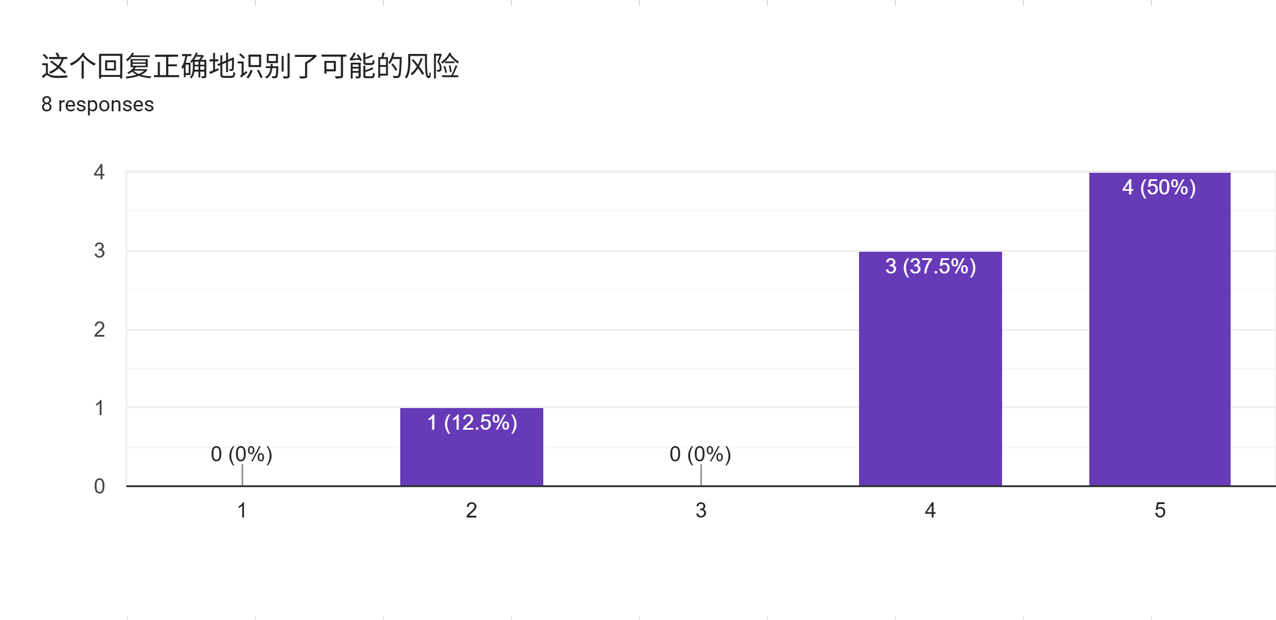
\includegraphics[width=0.45\linewidth]{correct.png}

	\caption{Participant evaluation results across key criteria}
	\label{fig:charts}
\end{figure}

As shown in Figure~\ref{fig:charts}, the system received consistently high ratings across the evaluated dimensions.

For relevance ("this response is reasonable" at top left), most of participants rated the responses as 4 or 5, indicating that the generated replies were generally appropriate and aligned with the original enquiry.

Similarly, tone appropriateness ("this response is professional" at top right) received strong evaluations, with most responses concentrated in the higher rating range. This suggests that the system is effective in maintaining a formal and suitable tone for business communication.

In terms of practicality ("this response helps advance cooperation" at bottom left), most participants provided positive ratings, indicating that the responses are not only correct but also useful in progressing real-world interactions. However, the presence of a small number of lower ratings suggests that some responses may lack sufficient actionability in more complex scenarios.

The system also performed well in risk identification ("this response correctly identifies potential risks" at bottom right), with the majority of participants agreeing that the risks that identified were correct and reasonable. This shows that the risk analysis module effectively captured important risk categories.

Qualitative feedback further supports these findings. Several participants noted that the system is highly effective for handling routine enquiries and can significantly improve communication efficiency.

However, some participants indicated that in more complex or suspicious scenarios, the system could provide clearer guidance or more decisive responses. This aligns with both the quantitative results and the observations in high- and critical-risk scenarios, where response strategies were sometimes perceived as insufficiently strong.

Overall, the results suggest that the system performs well in generating clear, professional, and generally useful responses, while highlighting opportunities for improvement in handling high-risk situations.

\section{System Revision Based on User Feedback}

The user study provided actionable insights that informed several improvements to the system.

First, the response generation prompts were refined to improve completeness and actionability. Based on user feedback, the system was updated to include clearer next steps, such as explicitly requesting missing information or proposing follow-up actions.

Second, tone consistency was strengthened. Although the system generally maintained a professional tone, prompt constraints were adjusted to ensure consistent politeness and formality across all scenarios.

Third, the risk-response mapping was improved. In particular, responses for high- and critical-risk scenarios were enhanced to be more explicit and context-aware. For example, the system was updated to more clearly decline or restrict engagement when strong risk indicators are present.

Finally, localisation behaviour was refined to better align response language and style with the inferred customer region, improving cross-cultural communication.

These improvements demonstrate how user feedback was directly integrated into both prompt design and system logic, leading to a more robust and reliable system.

% =========================
% Chapter 8
% =========================
\chapter{Discussion and Future Work}

\section{System-Level Reflection}

The proposed system, implemented as a prototype, represents a simplified version of a broader platform designed to support end-to-end international trade workflows. Beyond the implemented modules, the full architecture includes additional components such as market intelligence, customer prioritisation, and decision support.

This reflects a key insight that effective AI systems in real-world business contexts require coordinated integration across multiple functional domains, rather than isolated task-level automation. In international trade, communication, documentation, and risk assessment are inherently interdependent.

The extended architecture follows a three-layer structure comprising input, intelligent processing, and output layers, enabling scalable integration with enterprise systems.

This discussion is based on system design and evaluation results. While the communication and risk modules demonstrate strong performance in terms of fluency and structured output, there are still limitations in handling ambiguous inputs and achieving deeper module integration.

\section{Extension of Functional Modules}

While this project focuses on communication generation and risk identification, the broader system design envisions a set of additional modules that extend the system from an operational assistant to a decision-support platform. These modules are conceptual and are intended to illustrate the potential scalability of the architecture.

At a high level, the extended system would incorporate capabilities such as market awareness, customer relationship management, and decision support. These functions would enable the system to move beyond task execution towards supporting strategic business processes.

In addition, continuous risk monitoring could provide dynamic awareness by capturing evolving interaction patterns and external conditions.

Overall, these extensions reflect a transition from isolated functionalities to an integrated, platform-oriented system capable of supporting complex and interdependent workflows.

\section{Strengths of the Integrated Approach}

The integrated design provides several advantages.

It enables end-to-end workflow support, covering the process from enquiry handling to decision-making. It also improves contextual consistency by allowing information to be reused across modules, reducing redundancy.

Furthermore, the modular architecture supports incremental development, and the inclusion of structured outputs facilitates human-in-the-loop decision-making, enhancing rather than replacing human judgement.

\section{Limitations}

Despite its potential, several limitations remain.

The current system focuses primarily on communication and risk modules, while other components are underdeveloped. In particular, the document generation module remains limited, lacking a comprehensive set of standardised templates aligned with international legal and regulatory requirements. Therefore, the generated document is more suitable as a reference rather than a fully compliant document.

Integration between modules is also limited, and more advanced coordination mechanisms are required to fully realise system-level benefits. In addition, advanced functionalities would require reliable external data sources, which are not currently integrated.

The reliance on large language models introduces inherent limitations, including hallucination and variability in output quality, which cannot be fully eliminated by prompt optimisation.

Finally, increasing system complexity raises challenges in scalability and maintainability.

\section{Ethical, Legal and Social Considerations}

The expansion of the system into a decision-support platform raises a number of ethical, legal, and practical considerations, particularly in relation to the use of AI-generated outputs in business communication.

From a research ethics perspective, the project included a small-scale user study to evaluate system behaviour and usability. Participation was voluntary, and no sensitive personal data was collected. The study did not involve vulnerable groups or high-risk scenarios, and therefore ethical risks were considered minimal.

One key issue is the balance between automation and human control. As the system begins to provide strategic recommendations, there is a risk that users may over-rely on automated outputs without sufficient critical evaluation. For this reason, the system is designed to support, rather than replace, human decision-making.

Another concern is transparency. More complex modules, particularly those involving aggregated decision-making or risk assessment, may reduce the interpretability of system outputs. Ensuring that users have a basic understanding of how recommendations are generated is important to maintain trust and appropriate use.

In addition, the integration of risk assessment into communication introduces potential implications for business relationships. Automated restrictions or cautious responses may affect trust and negotiation dynamics, particularly when compliance considerations influence communication behaviour.

Data protection and privacy are also important considerations. The system processes textual inputs that may contain commercially sensitive information. To mitigate potential risks, the system is designed with limited data persistence, and no personal or confidential data is intentionally stored beyond what is necessary for system functionality. This follows the principle of data minimisation and reduces the likelihood of unintended exposure.

From a legal perspective, the system operates in a domain that may involve international trade regulations. However, it does not provide legal advice, and there is a potential risk that users may rely on generated outputs without independent verification. As such, the system should be understood as a decision-support tool rather than a substitute for professional judgement.

Overall, while the ethical and legal risks associated with this project are relatively limited due to its prototype nature, these considerations highlight the importance of responsible use, transparency, and continued human oversight in AI-assisted decision-making systems.

\section{Future Work}

Future work will focus on extending the system towards a more comprehensive platform.

A key direction is the enhancement of the documentation module through the introduction of standardised templates adapted to different regulatory contexts, alongside automated compliance checking capabilities.

Improving module integration is also important. Developing a central coordination mechanism can facilitate more effective interaction between components. Additionally, integrating external data sources, such as obtaining regulatory updates and market information will enhance the system's accuracy.

Another important direction is the introduction of user modelling and behavioural learning. By studying historical interactions and preferences of users, the system could adapt communication strategies, distinguishing between established clients and new or higher-risk customers. It could also learn user-specific communication styles to generate more personalised responses.

Further evaluation in real-world scenarios is required to assess usability and effectiveness. In the longer term, the system may evolve into a platform supporting extensibility and industry-specific customisation, moving towards a data-driven and adaptive decision-support system.

\section{Summary}

This chapter has examined the broader system vision and its implications. While the prototype demonstrates the feasibility of integrating AI into trade communication workflows, its full potential lies in evolving into a multi-module, decision-support platform. Future work will focus on expanding functionality, improving integration, and validating the system in real-world contexts.

% =========================
% Chapter 9
% =========================
\chapter{Conclusion}

\section{Project Summary}

This dissertation has presented the design, development, and evaluation of an AI-driven trade communication assistant intended to support SMEs in international trade scenarios. The project was motivated by the practical challenges that SMEs face in cross-border business, including multilingual communication difficulties, limited access to standardised documentation support, and uncertainty in risk and compliance assessment.

To address these challenges, the project developed a prototype system centred on two core functionalities: communication generation and risk identification, with an additional document generation component implemented as supporting functionality. The system adopts a modular client-server architecture and combines trade fact extraction, risk analysis, decision routing, and response generation within a unified workflow.

The development process followed an iterative approach. Initial implementation established the basic system pipeline, while later refinement focused on improving prompt design, output quality, risk-aware behaviour, and system usability. Through pilot testing and user feedback, the system was progressively improved to generate more natural, professional, and context-aware responses.

The user study further demonstrated that the system is capable of producing effective responses across a range of trade scenarios. In particular, the results suggest that the system performs well in routine and medium-risk cases, although further improvement is needed in handling more complex and critical-risk situations.

\section{Main Contributions}

The main contributions of this project can be summarised as follows.

First, the project proposed and implemented an integrated prototype for trade communication support, combining message understanding, communication generation, and risk identification within a single workflow. This addresses a gap in existing solutions, which often focus on isolated tasks rather than coordinated support.

Second, the project developed a risk-aware communication mechanism in which generated replies are informed not only by message content, but also by structured trade facts and identified risk signals. This enables the system to produce responses that are more context-sensitive and better aligned with practical business requirements.

Third, the project demonstrated the importance of iterative refinement in LLM-based systems. Through pilot testing, prompt engineering, post-processing, and user feedback, the system was improved in terms of clarity, tone consistency, localisation, and practical usability.

Finally, the project provides a foundation for future work on broader AI-assisted trade support systems. Although the current implementation remains a prototype, it establishes a modular architecture that can be extended towards more advanced decision-support and documentation capabilities.

\section{Final Remarks}

Overall, this project shows that AI can be used not only to automate isolated business tasks, but also to support more integrated trade communication workflows. The findings suggest that combining communication generation with structured risk analysis can provide practical value, particularly for SMEs that may lack the resources or expertise to manage complex international interactions efficiently.

At the same time, the project also highlights the limitations of current prototype systems. Large language models remain imperfect, document support is not yet fully standardised, and deeper coordination between modules is still needed. For these reasons, the system should be understood as an assistive tool rather than a replacement for human judgement.

Despite these limitations, the project demonstrates the feasibility and potential of an AI-driven trade communication assistant. With further development, broader data integration, and more extensive real-world evaluation, such systems could evolve into valuable platforms for supporting SMEs in global trade.

% =========================
% Appendix
% =========================
\appendix

\chapter{User Study Materials}

\section{Survey Overview}

This appendix presents the questionnaire used in the user study. The survey was designed to evaluate how users assess trade-related inquiries, respond to them, and perceive AI-generated responses.

The questionnaire consists of multiple sections, including:
\begin{itemize}
    \item Participant language preference
    \item Scenario-based inquiry evaluation
    \item AI response assessment
    \item Comparative judgement between human and AI responses
    \item Overall system feedback
\end{itemize}

---

\section{Scenario Example}

\subsection{Email Scenario}

\textbf{Incoming Email:}

\begin{quote}
Dear Friend, \\
We need your products urgently. Payment will be made by USDT or Bitcoin only. Please send invoice immediately and use a private account for faster settlement. Waiting for your urgent reply.
\end{quote}

---

\subsection{Stage 1: User Assessment}

\textbf{Q1. What key information is missing and what are the potential risks in this inquiry?}

(Open-ended response)

\vspace{0.3cm}

\textbf{Q2. How would you respond to this inquiry? (Select all that apply)}

\begin{itemize}
    \item Ask for product specifications
    \item Ask for quantity
    \item Ask for destination country
    \item Ask for delivery address
    \item Ask for company or buyer identity
    \item Provide quotation
    \item Provide product information/catalog
    \item Request clarification before proceeding
    \item Refuse to proceed
    \item Other
\end{itemize}

\vspace{0.3cm}

\textbf{Q3. What potential risks do you identify? (Select all that apply)}

\begin{itemize}
    \item Compliance and legal risks
    \item Country/geopolitical risks
    \item Business environment risks
    \item Transaction and counterparty risks
    \item Intent and commercial risks
    \item No obvious risks
    \item Other
\end{itemize}

\vspace{0.3cm}

\textbf{Q4. How would you handle this inquiry?}

\begin{itemize}
    \item Proceed normally
    \item Proceed with caution (verification needed)
    \item Refuse to proceed
\end{itemize}

---

\subsection{Stage 2: AI Response Evaluation}

\textbf{AI-generated response:}

\begin{quote}
Dear Friend, \\
Thank you for your message. \\
However, to proceed with your request, we need more information to verify your order and ensure a secure transaction. Could you please provide details regarding your company, including your registered address and any relevant identification? \\
Looking forward to your prompt response. \\
Best regards.
\end{quote}

\vspace{0.3cm}

\textbf{Risk assessment provided by the system:}

\begin{itemize}
    \item Overall level: Critical
    \item Tags: incomplete buyer profile, possible scam pattern, suspicious urgency, unverified counterparty
\end{itemize}

\vspace{0.3cm}

\textbf{Q5. Please rate the following statements (1–5 Likert scale):}

\begin{itemize}
    \item The AI response is reasonable
    \item The AI response is professional
    \item The AI response helps advance the transaction
    \item The AI response appropriately considers risks
\end{itemize}

---

\subsection{Stage 3: Comparative Evaluation}

\textbf{Q6. Which response do you prefer?}

\begin{itemize}
    \item My own response
    \item AI-generated response
    \item Both are similar
\end{itemize}

\vspace{0.3cm}

\textbf{Q7. Do you agree with the system's risk assessment?}

\begin{itemize}
    \item Fully agree
    \item Partially agree
    \item Disagree
\end{itemize}

---

\section{Overall Feedback}

\textbf{Q8. Do you think this system is helpful? (1–5)}

\vspace{0.3cm}

\textbf{Q9. To what extent are you willing to use this system? (1–5)}

\vspace{0.3cm}

\textbf{Q10. How could the AI response be improved?}

(Open-ended response)

\vspace{0.3cm}

\textbf{Q11. Why are you willing or not willing to use this system?}

(Open-ended response)

% =========================
% References
% =========================
\clearpage
\renewcommand{\bibname}{References}

\begingroup
\setlength{\bibhang}{0pt}
\setlength{\bibsep}{0.5em}
\bibliographystyle{plainnat}

\begin{thebibliography}{99}

\bibitem[International Trade Centre(2021)]{itc2021}
International Trade Centre (2021) \textit{SME Competitiveness Outlook 2021: Empowering the Green Recovery}. Geneva: ITC. doi:10.18356/9789210057660.

\bibitem[McKinsey \& Company(2023)]{mckinsey2023}
McKinsey \& Company (2023) \textit{The Economic Potential of Generative AI: The Next Productivity Frontier}. McKinsey Global Institute. Available at: \url{https://www.mckinsey.com/capabilities/tech-and-ai/our-insights/the-economic-potential-of-generative-ai-the-next-productivity-frontier} (Accessed: 23 November 2025).

\bibitem[OECD(2017)]{oecd2017}
OECD (2017) \textit{Enhancing the Contributions of SMEs in a Global and Digitalised Economy}. Paris: OECD. Available at: \url{https://one.oecd.org/document/C/MIN(2017)8/en/pdf} (Accessed: 24 November 2025).

\bibitem[OECD(2021)]{oecd2021}
OECD (2021) \textit{The Digital Transformation of SMEs}. OECD Studies on SMEs and Entrepreneurship. Paris: OECD Publishing. doi:10.1787/bdb9256a-en.

\bibitem[OECD(2022)]{oecd_ai_trade}
OECD (2022) \textit{Artificial Intelligence and International Trade: Some Preliminary Implications}. OECD Trade Policy Papers No. 260. Paris: OECD Publishing. doi:10.1787/13212d3e-en.

\bibitem[OECD(2025)]{oecd_doc}
OECD (2025) \textit{The digitalisation of trade documents and processes: Going paperless today, going paperless tomorrow}. OECD Trade Policy Papers, No. 297. Paris: OECD Publishing. doi:10.1787/64872f25-en.

\bibitem[Ozturk(2024)]{ozturk2024}
Ozturk, O. (2024) ‘The Impact of Artificial Intelligence on International Trade: Opportunities and Challenges’, \textit{Economies}, 12(11), 298. doi:10.3390/economies12110298.

\bibitem[UNCTAD(2021)]{unctad2021}
UNCTAD (2021) \textit{Digital Economy Report 2021: Cross-border data flows and development – For whom the data flow}. Geneva: United Nations. Available at: \url{https://unctad.org/system/files/official-document/der2021_en.pdf} (Accessed: 12 January 2026).

\bibitem[World Bank(2020)]{worldbank2020}
World Bank (2020) \textit{Small and Medium Enterprises (SMEs) Finance}. Available at: \url{https://www.worldbank.org/en/topic/smefinance} (Accessed: 10 January 2026).

\bibitem[World Trade Organization(2016)]{wto2016}
World Trade Organization (2016) \textit{World Trade Report 2016: Levelling the Trading Field for SMEs}. Geneva: WTO. Available at: \url{https://www.wto-ilibrary.org/content/books/9789287045003} (Accessed: 10 January 2026).

\bibitem[World Trade Organization(2025)]{wto2025}
World Trade Organization (2025) \textit{World Trade Report 2025: Making trade and AI work together to the benefit of all}. Geneva: WTO. Available at: \url{https://www.wto-ilibrary.org/content/books/9789287074560} (Accessed: 10 January 2026).

\end{thebibliography}
\endgroup

\end{document}